By selecting e$^{+}$e$^{-}$ pairs from the triggered events we are able to study basic distributions of pair production kinematics and in particular those related to our vertex performance. Pairs of opposite charge tracks, one in the top and one in the bottom half of the SVT, with larger than 400~MeV were selected. The pair production kinematics are relatively well reproduced given the alignment of the tracker; Fig.~\ref{fig:pair_kin} shows the invariant mass and ratio of electron momentum over the sum of electron and positron. 
\begin{figure}[ht]
   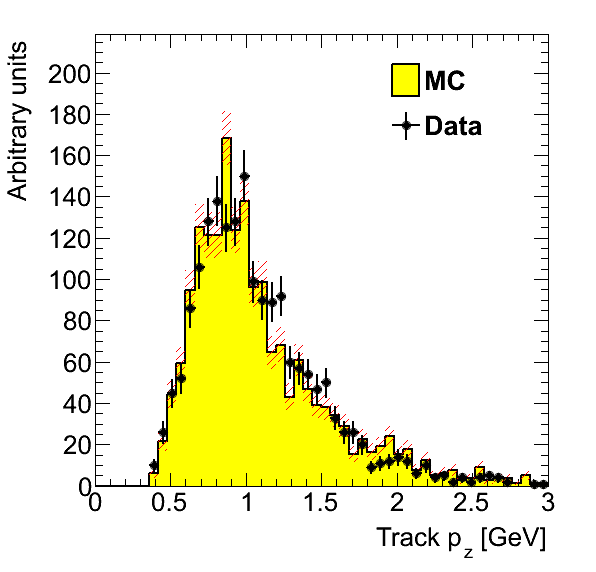
\includegraphics[scale=0.25]{test2012/vertexing/figures/h_trk_top_px_h_trk_top_px_trigseltwotrksel4hit_recoilmc_twotrkfilt.png}
   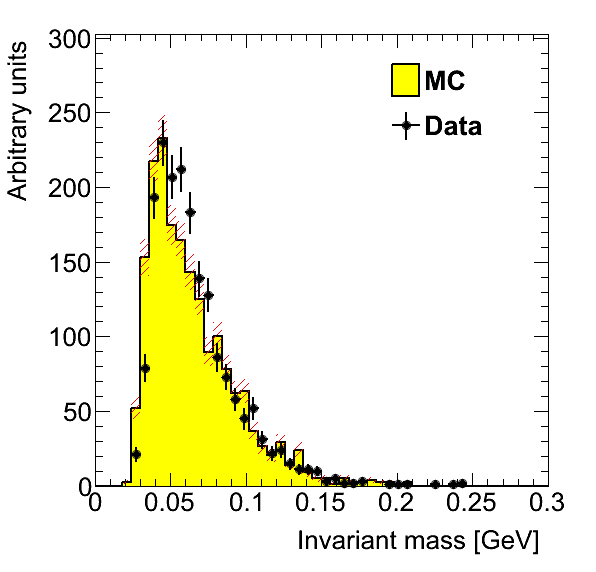
\includegraphics[scale=0.25]{test2012/vertexing/figures/h_invM_h_invM_dataMC_trigseltwotrksel4hit_recoilmc_twotrkfilt.png}
   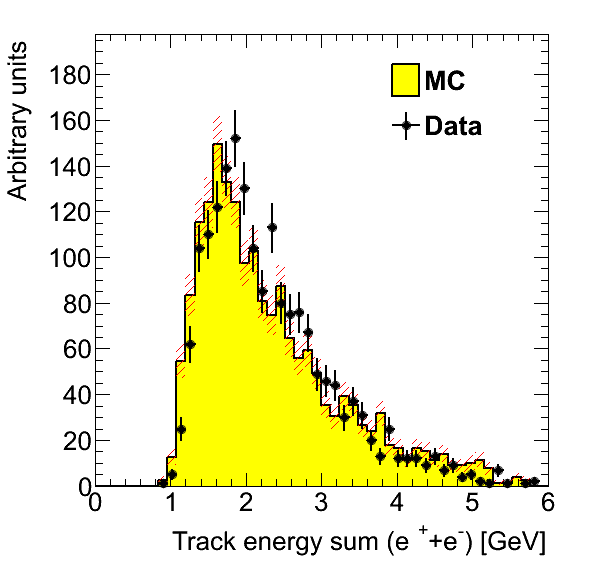
\includegraphics[scale=0.25]{test2012/vertexing/figures/h_sumE_h_sumE_dataMC_trigseltwotrksel4hit_recoilmc_twotrkfilt.png}
%   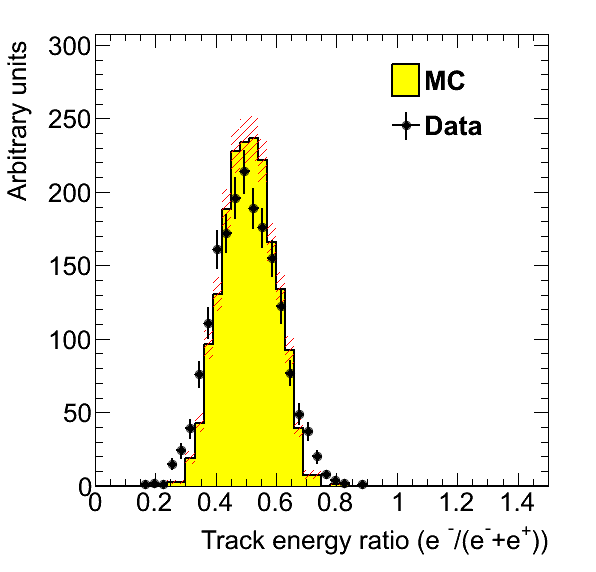
\includegraphics[scale=0.25]{test2012/vertexing/figures/h_ratioEsum_h_ratioEsum_dataMC_trigseltwotrksel4hit_recoilmc_twotrkfilt.png}
\caption{\small{Kinematic distributions for e$^+$e$^-$ pairs selected by opposite charged tracks in the top and bottom half of the tracker: track momentum in the top half of the SVT (left), invariant mass (middle) and the sum of the track momentum for the pair.}} 
\label{fig:pair_kin}
\end{figure}

For the vertexing 
performance the foremost difference compared to electron beam running is that the target was 
located $\sim67$~cm from our nominal target position; giving almost collinear tracks in the detector. This 
degrades the vertex resolution along the 
beam line compared to that expected in an electron beam with tracks from the nominal target position. 
Furthermore, tails of the vertex distributions are impossible to study with the finite sample of events from the 
Test Run. 
Nevertheless, useful information can still be 
obtained by studying the vertex distributions. Figure~\ref{fig:vtx_pos} shows the distance of closest 
approach of the momentum vectors extrapolated in the 
upstream direction from our analyzing magnet, taking into account the measured fringe field. 
 \begin{figure*}[t]
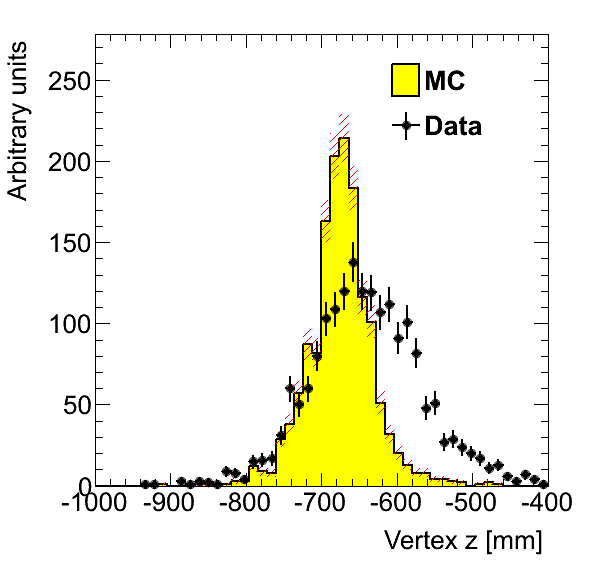
\includegraphics[ scale=0.25]{test2012/vertexing/figures/h_vtx_fr_x_h_vtx_x_dataMC_trigseltwotrksel4hit_recoilmc_twotrkfilt.png}
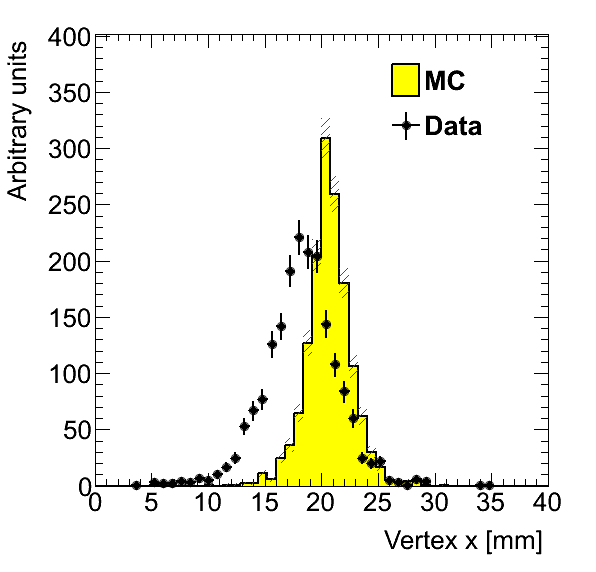
\includegraphics[ scale=0.25]{test2012/vertexing/figures/h_vtx_fr_y_h_vtx_y_dataMC_trigseltwotrksel4hit_recoilmc_twotrkfilt.png}
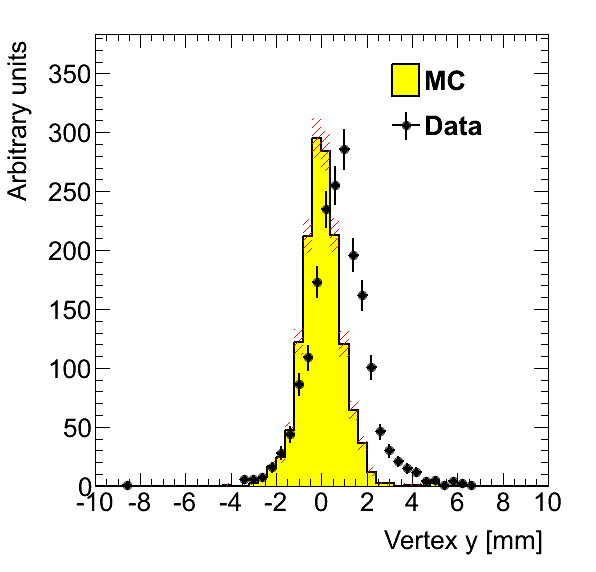
\includegraphics[ scale=0.25]{test2012/vertexing/figures/h_vtx_fr_z_h_vtx_z_dataMC_trigseltwotrksel4hit_recoilmc_twotrkfilt.png}
\caption{\small{Vertex position represented by the distance of closest approach of the extrapolated momentum vectors upstream of the analyzing magnet. The overall shift from zero in the x-direction is due to a 30~mrad rotation of the SVT with respect to the beam line.}}\label{fig:vtx_pos}
\end{figure*}
While the tails of the vertex distribution expected in electron beam running is not accessible here the 
fact that the core is relatively well described provides confidence of the description of the amount of 
material and the multiple scattering description.  These are crucial for benchmarking the physics reach of the 
HPS detector since both the mass and vertex resolution that determine the physics reach are limited by multiple scattering.

